\documentclass{article}
\usepackage[utf8]{inputenc}
\usepackage[T1]{fontenc}
\usepackage[english]{babel}
\setlength{\parindent}{0pt}
\usepackage{hyperref}
\hypersetup{
    colorlinks=true,
    linkcolor=blue,
    filecolor=magenta,      
    urlcolor=cyan}
\usepackage{graphicx}
\graphicspath{ {./pic/} }
\usepackage{multicol}
\usepackage{lscape}

\usepackage{fourier,amssymb,microtype,amsmath,gensymb}
\newcommand{\R}{\mathbb{R}}
\usepackage{mdframed,caption,xcolor}
\usepackage{tikz,tkz-euclide}

\title{Seminar 5. Production Theory}
\author{Xiaoguang Ling \\  \href{xiaoguang.ling@econ.uio.no}{xiaoguang.ling@econ.uio.no}}
\date{\today}

\begin{document}

\maketitle

%%%%%%%%%%%%%%%%%%%%%%%%%%%%%%%%%%%%%%%%%%%%%%%%%%%%%%%%%%%%%%%%%%%%%%%%%%%%%%%%%%%%%%%%%%%%%%
\begin{landscape}
\section*{Production Duality}

\vspace{3mm}

\begin{mdframed}[backgroundcolor=blue!20,linecolor=white]
The dual relation between product maximization problem and cost minimization problem is simpler than consumers' theory. 

\begin{itemize}
\item Given $y = f(x)$, profit function is only a function of $x$. That's why minimizing the cost will maximize the profit at the same time.
\end{itemize}

\end{mdframed}

\vspace{3mm}
{\scriptsize
\usetikzlibrary{arrows.meta}
\tikzset{%
  >={Latex[width=1mm,length=1mm]},
  % Specifications for style of nodes:
            base/.style = {rectangle, rounded corners, draw=black,
                           minimum width=2cm, minimum height=1cm,
                           text centered, font=\sffamily},
  Starts/.style = {base, fill=blue!30},
         process/.style = {base, minimum width=2.5cm, fill=orange!15,
                           font=\ttfamily},
}
\begin{tikzpicture}[node distance=2cm,
every node/.style={fill=white, font=\sffamily}, align=center]
\node (start) [Starts] {Profit Maximization: \\ $\max_{(x,y) \ge 0} \ py - wx, s.t. y \le f(x)$};
\node (1) [process, below of=start] {Output Supply Function: \\ $y^* \equiv y(p,w)$ \\ Input Demand Functions: \\ $x^* \equiv x(p,w)$};
\node (2) [process, below of=1] {Profit Function: \\ $\pi (p,w) =  py^* - wx^*$};

\node (3) [process, left of=2,xshift=-1.5cm,yshift=1cm]  {Hotelling's lemma (pp.148): \\ $y(p,w) = \frac{\partial \pi(p,w)}{\partial p}$ \\  \\   $x_i(p,w) = - \frac{\partial \pi(p,w)}{\partial w_i}$};


\draw[->]  (start) -- (1);
\draw[->] (1) -- (2);
\draw[dashed]  (2) --  (3);
\draw[dashed]  (3) --  (1);


{\tiny
\path (start) to  node {Let $y = f(x)$, solution $x^*, y^*$} (1); 
\path (1) to  node {maximized value} (2); 
}
  
%%%%%%%%%%%%%%%%%%%%%%%%%%%%%%%%%%%%%%%%%%%%%%%%%%%%%%%%%%%%%%%%%%%%%%%%%%%%%%%%%%%%%%%%%%%%%%%%%%%%%%%%%%%%%

\node (start2) [Starts, right of = 1, xshift =6cm, yshift=2cm] {Cost Minimization: \\ $\min_{x \in \R^n_+} \ w x, s.t. f(x) \ge y$};
\node (21) [process, below of=start2] {Conditional Input Demand: \\ $x(w,y)$};
\node (22) [process, below of=21] {Cost Function: \\ $c(w,y) = w x(w,y)$};
\node (23) [process, right of=22,xshift=1.5cm,yshift=1cm]  {Shephard's lemma(pp.138): \\ $x_i(w^0,y^0) = \frac{\partial c(w^0,y^0)}{\partial w_i}$};
\node (24) [process, below of=22] {Production Function (pp.144): \\ $f(x) \equiv max\{y \ge 0 | wx \ge c(w,y), \forall w \gg 0 \}$};
\draw[->]  (start2) -- (21);
\draw[->]  (21) -- (22);
\draw[dashed]  (22) --  (23);
\draw[dashed]  (23) --  (21);
\draw[->] (22) --  (24);
{\tiny
\path (start2) to  node {Let $f(x) = y$,solution $x^*$} (21); 
\path (21) to  node {minimized value} (22); 
}
%%%%%%%%%%%%%%%%%%%%%%%%%%%%%%%%%%%%%%%%%%%%%%%%%%%%%%%%%%%%%%%%%%%%%%%%%%%%%%%%%%%%%%%%%%%%%%%%%%%%%%%%%%%%
\node (31) [process, right of=1,xshift=2cm,yshift=0.8cm] {FOC(pp.146): \\ $\frac{\partial f(x^*) / \partial x_i}{\partial f(x^*) / \partial x_j} = \frac{w_i}{w_j}$ \\ Given: \\ $f(x) = y$};


\draw[<-]  (2) --  (22);
\draw[<->]  (1) --  (21);

\path (22) to  node[above] {$\pi (p,w) = py(p,w) - c(w, y(p,w))$}  (2); 




\end{tikzpicture}
}
\end{landscape}

%%%%%%%%%%%%%%%%%%%%%%%%%%%%%%%%%%%%%%%%%%%%%%%%%%%%%%%%%%%%%%%%%%%%%%%%%%%%%%%%%%%%%%%%%%%%%%

\section{Jehle \& Reny 3.35}

Calculate the \textbf{cost function} and the \textbf{conditional input demands} for the linear production function,
$y = \Sigma^n_{i=1} \alpha_i x_i$.

\begin{mdframed}[backgroundcolor=blue!20,linecolor=white]

\textbf{Production Function}(Jehle \& Reny pp.127)

We use a function $y = f(x)$ to denote $y$ units of a certain commodity is produced using input $x$, where $x \in \R^n_+, y \in \R^1_+$

\vspace{2mm}

\textbf{ASSUMPTION 3.1 Properties of the Production Function} (Jehle \& Reny pp.127)

The production function, $f : \R^n_+ \to \R_+$ , is continuous, strictly increasing, and strictly
quasiconcave on $\R^n_+$, and $f (0) = 0$.

\vspace{2mm}

\textbf{DEFINITION 3.5 The Cost Function} (Jehle \& Reny pp.136)

The cost function, defined for all input prices $w \gg 0$ and all output levels $y \in f(\R^n_+)$ is the
minimum-value function,
$$c(w,y) \equiv \min_{x \in \R^n_+} w \cdot x , \ \ s.t. \ \ f(x) \ge y.$$
The solution $x(w, y)$ is referred to as the firm’s \textbf{conditional input demand}, because it is conditional on the level of output $y$.

\begin{itemize}
\item  \textbf{Conditional input demand} is similar to Hicksian demands for consumers.
\end{itemize}

\end{mdframed}

\vspace{2mm}

\begin{mdframed}[backgroundcolor=blue!20,linecolor=white]

Here the linear production function $y = \Sigma^n_{i=1} \alpha_i x_i$ is very similar to the "\textbf{perfect substitution}" preference in Seminar 4.

\begin{itemize}

\item  The product can be produced by any input $x_i$, the only difference is that for each unit of input, different $x_i$ produces different amount $\alpha_i$ of the output. 

\item  The Marginal Rate of Technical Substitution of input $x_j$ for input $x_i$ is constant: $MRTS_{ij} = \frac{\partial f(x)/ \partial x_i}{\partial f(x)/ \partial x_j} = \frac{\alpha_i}{\alpha_j}$.

\end{itemize}

An example: an apple jam factory has 2 types of input, "single apple ($x_1$)" and "2-apple pack ($x_2$)".

\begin{itemize}
\item With a "single apple", the factory can produce a bottle of apple jam;
\item with a "2-apple pack", 2 bottles.
\item The production function is $y = 1 \cdot x_1 + 2 \cdot x_2$
\end{itemize}

How will the factory choose? Similarly to consumers' preference substitution preference, the factory will spend all money on the "cheapest per unit (of output)" input. 

Denote the price for $x_1$ and $x_2$ as $w_1$, $w_2$
\begin{itemize}
\item If $\frac{w_1}{1} = \frac{w_2}{2}$, the factory doesn't care which to use;
\item If $\frac{w_1}{1} < \frac{w_2}{2}$, single apple is cheaper;
\item If $\frac{w_1}{1} > \frac{w_2}{2}$, 2-apple pack is cheaper.
\end{itemize}

\end{mdframed}


Denote the price for input $x_i$  as $w_i$. Define $\omega = min \{\frac{w_1}{\alpha_1}, \frac{w_2}{\alpha_2}, \dots ,\frac{w_n}{\alpha_n}\} $

\vspace{2mm}

If $\omega$ is the price of only one input $x_j$, the firm will only use input $x_j$ to minimize its cost. 

\begin{itemize}
\item Thus $y = \alpha_j x_j$ can minimize the cost, and $x_j = \frac{y}{\alpha_j}$ is the conditional input demands.
\item The cost function $c(w,y) = w_j \frac{y}{\alpha_j} = \omega y$.
\end{itemize}


If $\omega$ is the price of several inputs $x_m, m = 1,2, \dots, M$, the firm can freely combine $x_m$ to minimize its cost, as long as  $\Sigma^M_{m=1} \alpha_m x_m = y$.

\vspace{2mm}

For cost funtion, since $\frac{w_1}{\alpha_1} = \frac{w_2}{\alpha_2}= \dots =\frac{w_M}{\alpha_M} = \omega$, $\omega$ is the price for $1$ single apple (the input needed to produce $1$ bottle of jam), for example. Again, to produce $y$ bottles of jam, you need the same number ($y$) of single apples. The cost function is thus $\omega y$

%%%%%%%%%%%%%%%%%%%%%%%%%%%%%%%%%%%%%%%%%%%%%%%%%%%%%%%%%%%%%%%%%%%%%%%%%%%%%%%%%%%%%%%%%%%%%%
\section{Another production \& cost function example from exam 2019 Q1(b): HydroP}

To produce electricity $E$, firm HydroP uses water $W$ and a plant $P$ as
main inputs. It operates in a unique location, so that no further plants can be
built. Without the plant the production is $0$. With the plant, electricity can be
produced according to the following production function:


\begin{equation}
E=
    \begin{cases}
0, \ \ \ \ if \ \ W \le \underbar{W} \\
4W, \ \ \ \ if \ \   \underbar{W} \le   W \le \bar{W} \\
3\bar{W}, \ \ \ \ if \ \ \bar{W} < W \\
    \end{cases}
    \label{eq:hydro}   
\end{equation}

%***************************************************
\subsection{a) Function property}

\textbf{ [5\%] Is this production function: continuous? (strictly) increasing? (strictly) quasiconcave? increasing/decreasing/constant returns
to scale?}

\begin{mdframed}[backgroundcolor=blue!20,linecolor=white]

When $W = \underbar{W}$, the production function value is $0$ and $4\underbar{W}$. Therefore $\underbar{W} = 0$.

But the guideline online treated "$W \le \underbar{W}$" as "W < \underbar{W}", which is incorrect.

\begin{center}
\begin{tikzpicture}[scale=1]
\draw[thick,<->] (0,9) node[left]{$E$} -- (0,6) node[left]{$3\bar{W}$} --(0,0)--(2,0)node[below]{$\bar{W}$} -- (4,0) node[below,blue]{Too much water}--(6,0) node[right]{$W$};
\draw[thick] (-5,0) --(0,0);
\draw[thick] (0,-1) -- (0,-0.3)node[right]{$0(\underbar{W})$} --(0,0);
\draw[thick, blue] (-4,0) -- (-2.2,0)node[below]{Water below the turbine} --(0,0) ;
\draw[thick, blue] (0,0) -- (2,8);
\draw[thick, blue] (2,6) -- (5,6);
\draw[dashed] (2,8.5) -- (2,0);
\draw[fill,blue] (2,8) circle [radius =0.06];
\draw [blue]  (2,6) circle [radius =0.06];
\end{tikzpicture}
\captionof{figure}{HydroP's Production function}
\label{fig:hydro}
\end{center}
\vspace{2mm}

Obviously, the production function is:
\begin{itemize}
\item not continuous at $(\bar{W},0)$
\item not increasing in $(-\infty,0)$ and $(\bar{W},+\infty)$
\item quasiconcave: $f (x^t) \ge min[f (x^1), f (x^2)]$ for all $t ∈ [0, 1]$.
\item not strictly quasiconcave: sometimes $f (x^t) = min[f (x^1), f (x^2)]$
\item return to scale (pp.132 $f(tx) \ ? \ tf(x)$) uncertain, "jump" around $(0,0)$ and $(\bar{W},0)$
\end{itemize}
\end{mdframed}

Answer:

The production function is:
\begin{itemize}
\item not continuous
\item not increasing and therefore not strictly increasing
\item quasiconcave but not strictly quasiconcave
\item return to scale uncertain, sometimes increase, sometimes constant or decrease.
\end{itemize}


\begin{mdframed}[backgroundcolor=yellow!20,linecolor=white]
\begin{itemize}
\item Draw sketch for unusual function!
\item Don't be wordy, don't prove unnecessarily 
\end{itemize}
\end{mdframed}

%***************************************************
\subsection{b) Cost function}

\textbf{[7\%] Determine the cost function for this firm (let the price of
water be and let K be the cost of the plant). Is the cost function
continuous?}

\begin{mdframed}[backgroundcolor=blue!20,linecolor=white]
Cost function: $c(w,y) \equiv \min_{x \in \R^n_+} w \cdot x , \ \ s.t. \ \ f(x) \ge y.$

\begin{itemize}
\item It is always the minimized value function
\item It's a function of input price $w$ and output amount $y$
\item There can be fixed cost in the short run.
\end{itemize}

In this question, the only input is water, with a price of $p_w$. There is also a fixed cost $K$ if you
build the plant. The output is electricity $E$. We can write the cost function as $c(p_w,K,E)$

\vspace{3mm}

Now let's find the miminum cost with different output amount $E$ on our sketch.

\vspace{3mm}

\textbf{When $E=0$}, you will not build the plant to minimize your cost, $c(p_w,K,0) = 0$

\vspace{3mm}

\textbf{When $E \in (0,4\bar{W}]$}, you must build the plant with a fixed cost $K$. Besides, for any output $E$, you need  $\frac{E}{4}$ water,
which costs $p_w\frac{E}{4}$.

\begin{itemize}
\item Can you produce more than $4\bar{W}$? No, that's not allowed by your technology, the plant.
\item Will you use water more than $\bar{W}$? No, that's not cost minimized. You always choose the most
"economical" way to minimize the cost. Don't forget you're looking for the \textbf{cost function}
\end{itemize}

\end{mdframed}


The cost function is:


\begin{equation}
c(p_w,K,E)=
    \begin{cases}
0, \ \ \ \ if \ \ E = 0 \\
K + p_w\frac{E}{4}, \ \ \ \ if \ \   0 <  E \le 4\bar{W} \\
    \end{cases}
    \label{eq:hydro_c}   
\end{equation}


\begin{mdframed}[backgroundcolor=blue!20,linecolor=white]
Again, note $\underbar{W} = 0$. Compare the result with the \href{https://www.uio.no/studier/emner/sv/oekonomi/ECON4220/previous-exams/econ32_4220_2019h_sensorveiledning.pdf}{online guideline}. 

\begin{itemize}
\item Based on the guideline's understanding of the question, is it possible to produce $E \in (0, 4\underbar{W})$
\end{itemize}
\end{mdframed}

\begin{mdframed}[backgroundcolor=yellow!20,linecolor=white]
Many students lost points because they didn't know what is the "variable" of a cost function $c(w,y)$.

\begin{itemize}
\item A common mistake is: $c = \dots , \ if \ \ W \in (0,3\bar{W})$. Note $W$ is input (water) amount, not a variable of cost function.
\item Ask yourself, what is the input price $w$ here? What is the product amount $y$ here?

\end{itemize}


\end{mdframed}


%***************************************************
\subsection{c) Integrability}
\textbf{ [5\%] Can one recover the original production function from the
cost function? Why not?}

\begin{mdframed}[backgroundcolor=blue!20,linecolor=white]
Observe function \ref{eq:hydro_c}, can you guess what is the production function $f(x)$?

\textbf{When $E=0$}, there is no cost and no output, $f(0) = 0$

\textbf{When $E \in (0,4\bar{W}]$}, we know $K$ is fixed cost, $p_w$ is the price of your input,  $\frac{E}{4}$ is the
amount of water you used to generate electricity (output) $E$. Thus $$f(\frac{E}{4}) = E \Rightarrow f(x) = 4x$$

\begin{itemize}
\item Can you know the production function is $f(x) = 3\bar{W}$ when $x > \bar{W}$? No, you can't imagine that from the cost function.
\item Since cost function is always the minimized value function, the production function recovered from a cost function is only the "most efficient" part. Any non- cost -minimization technology can't be recovered. 
\end{itemize}
\end{mdframed}


No. Because when $x > \bar{W}$, the production is never cost minimizing, while  cost function can only reflect the technology minimizing the cost.

%%%%%%%%%%%%%%%%%%%%%%%%%%%%%%%%%%%%%%%%%%%%%%%%%%%%%%%%%%%%%%%%%%%%%%%%%%%%%%%%%%%%%%%%%%%%%%
\section{Jehle \& Reny 3.46}

\begin{itemize}
\item Verify Theorem 3.7 for the profit function obtained in Example 3.5. 
\item Verify Theorem 3.8 for the associated output supply and input demand functions.
\end{itemize}
%***************************************************
\subsection{Verify Theorem 3.7}

\begin{mdframed}[backgroundcolor=blue!20,linecolor=white]

\textbf{DEFINITION 3.7 The Profit Function} (Jehle \& Reny pp.148)

$$\pi (p,w) \equiv \max_{(x,y) \ge 0} py - wx, \ \ s.t. y \le f(x)$$

\textbf{Note,} $y \le f(x)$ means "you can only decide to produce what's possible to be produced":

\begin{itemize}
\item Assume you want to set an optimal output $y$, forget input $x$ for now;
\item You can "waste", i.e., output $y < f(x)$ is possible. Input is not efficiently used for technology $f(x)$;
\item You can't produce more than what your technology $f(x)$ allows, i.e.  $y \ngtr f(x)$.
\end{itemize}

It's not easy to solve the maximization problem directly because there are 2 variable, $y$ and $x$ (again, $y$ is \textbf{NOT} 
necessarily to be $f(x)$, but it can't exceed $f(x)$).

Since to waste will definitely reduce profit (you have some cost but don't produce anything), as a price reveiver, you will always avoid wasting by
making fully use of your technology, i.e. $y = f(x)$. Then the profit maximization problem is transformed into:

$$\pi (p,w) = \max_{x \ge 0} p f(x) - wx$$

No constraint anymore! The function has only one variable, input $x$. FOC will (usually) solve the problem.

\end{mdframed}

\vspace{2mm}

\begin{mdframed}[backgroundcolor=blue!20,linecolor=white]

In \textbf{Example 3.5} (Jehle \& Reny pp.151), the CES production function is:

$$y = (x_1^\rho + x_2^\rho)^{\frac{\beta}{\rho}}$$

Where $\beta < 1$ and $0 \ne \rho <1$. To obtain the profit function, we need to solve the maximization problem:


$$\max_{(x,y) \ge 0} py - wx, \ \ s.t. \ \ y \le (x_1^\rho + x_2^\rho)^{\frac{\beta}{\rho}}$$

Again, we don't waste, i.e. $ y = (x_1^\rho + x_2^\rho)^{\frac{\beta}{\rho}}$, the problem above is then:

$$\max_{x \ge 0} p(x_1^\rho + x_2^\rho)^{\frac{\beta}{\rho}} - w_1x_1 - w_2x_2$$

FOC are given in the textbook pp. 151. 

The $y^*$ solved is the \textbf{output supply function}:
\begin{equation}
y^* = (p\beta)^{-\frac{\beta}{\beta - 1}}(w_1^r + w_2^r)^{\frac{\beta}{r(\beta - 1)}}
    \label{eq:E5}   
\end{equation}

(You'll compare the output function with equation \ref{eq:check1} derived from cost minimization.)

The $x^*$ solved is the \textbf{input demand function}:

\begin{equation}
x_i^* = w_i^{\frac{1}{\rho -1}}  (p\beta)^{\frac{-1}{\beta - 1}}(w_1^r + w_2^r)^{\frac{\rho -\beta}{\rho(\beta -1)}}
    \label{eq:E6}   
\end{equation}



The profit function is thus:
\begin{equation}
\pi = py^* - wx^* = p^{-\frac{1}{\beta - 1}} (w_1^r + w_2^r)^{\frac{\beta}{r(\beta - 1)}}\beta^{-\frac{\beta}{\beta - 1}}(1-\beta)
    \label{eq:E7}   
\end{equation}

(You'll compare the profit function with equation \ref{eq:check2} derived from cost minimization.)

\end{mdframed}

\vspace{2mm}

\begin{mdframed}[backgroundcolor=blue!20,linecolor=white]

\textbf{THEOREM 3.7 Properties of the Profit Function} (Jehle \& Reny pp.148)

If $f$ satisfies Assumption 3.1, then for $p \ge 0$ and $w \ge 0$, the profit function $\pi (p,w)$, where well-defined, is continuous and

\begin{enumerate}

\item Increasing in $p$,
\item Decreasing in $w$,
\item Homogeneous of degree one in $(p,w)$,
\item Convex in $(p,w)$,
\item Differentiable in $(p,w)$.
\item Moreover, under the additional assumption that $f$ is strictly concave \\ (Hotelling's lemma),

$$y(p,w) = \frac{\partial \pi(p,w)}{\partial p},\ and \ \ x_i(p,w) = - \frac{\partial \pi(p,w)}{\partial w_i}. \ \ \ \ i = 1,2, \dots , n.$$
\end{enumerate}
\end{mdframed}

\textbf{1.Increasing in $p$}

For $\pi(p,w) = py^* - wx^* = p^{-\frac{1}{\beta - 1}} (w_1^r + w_2^r)^{\frac{\beta}{r(\beta - 1)}}\beta^{-\frac{\beta}{\beta - 1}}(1-\beta)$,
\begin{align*}
\frac{\partial \pi(p, w)}{\partial p} &= (-\frac{1}{\beta - 1})p^{-\frac{1}{\beta - 1}-1} (w_1^r + w_2^r)^{\frac{\beta}{r(\beta - 1)}}\beta^{-\frac{\beta}{\beta - 1}}(1-\beta) \\
&= p^{\frac{\beta}{1 - \beta}} (w_1^r + w_2^r)^{\frac{\beta}{r(\beta - 1)}}\beta^{-\frac{\beta}{\beta - 1}} \\
&= (p\beta)^{\frac{\beta}{1 - \beta}} (w_1^r + w_2^r)^{\frac{\beta}{r(\beta - 1)}}
\end{align*}

When $0<\beta <1$, $\frac{\partial \pi(p, w)}{\partial p} \ge 0 $

\vspace{3mm}
\textbf{2.Decreasing in $w$}

\begin{align*}
\frac{\partial \pi(p, w)}{\partial w_i} &= 
p^{-\frac{1}{\beta - 1}} [\frac{\beta}{r(\beta - 1)}](w_1^r + w_2^r)^{\frac{\beta}{r(\beta - 1)} -1} r w_i^{r-1}\beta^{-\frac{\beta}{\beta - 1}}(1-\beta) \\
&= p^{-\frac{1}{\beta - 1}} [-\beta](w_1^r + w_2^r)^{\frac{\beta}{r(\beta - 1)} -1} w_i^{r-1}\beta^{-\frac{\beta}{\beta - 1}} \\
&= p^{-\frac{1}{\beta - 1}} [-1](w_1^r + w_2^r)^{\frac{\beta}{\frac{\rho}{\rho -1}(\beta - 1)} -1} w_i^{\frac{\rho}{\rho -1}-1}\beta^{1-\frac{\beta}{\beta - 1}} \\
&= -p^{-\frac{1}{\beta - 1}}(w_1^r + w_2^r)^{\frac{\beta}{\frac{\rho}{\rho -1}(\beta - 1)} -1} w_i^{\frac{1}{\rho -1}}\beta^{-\frac{1}{\beta - 1}} \\
&= -(p\beta)^{-\frac{1}{\beta - 1}}(w_1^r + w_2^r)^{\frac{(\rho -1)\beta}{\rho(\beta - 1)} -1} w_i^{\frac{1}{\rho -1}}\\
&= -(p\beta)^{-\frac{1}{\beta - 1}}(w_1^r + w_2^r)^{\frac{\rho -\beta}{\rho(\beta-1)} }w_i^{\frac{1}{\rho -1}}
\end{align*}

$i = 1,2$.

When $0<\beta <1$, $\frac{\partial \pi(p, w)}{\partial w_i} \le 0 $

\vspace{3mm}
\textbf{3.Homogeneous of degree one in $(p,w)$}

\begin{align*}
\pi(tp,tw) &= (tp)^{-\frac{1}{\beta - 1}} [(tw_1)^r + (tw_2)^r]^{\frac{\beta}{r(\beta - 1)}}\beta^{-\frac{\beta}{\beta - 1}}(1-\beta) \\
&= t^{-\frac{1}{\beta - 1}}p^{-\frac{1}{\beta - 1}} t^{\frac{\beta}{(\beta - 1)}} [(w_1)^r + (w_2)^r]^{\frac{\beta}{r(\beta - 1)}}\beta^{-\frac{\beta}{\beta - 1}}(1-\beta) \\
&= t^{-\frac{1}{\beta - 1} + \frac{\beta}{(\beta - 1)}}p^{-\frac{1}{\beta - 1}} [(w_1)^r + (w_2)^r]^{\frac{\beta}{r(\beta - 1)}}\beta^{-\frac{\beta}{\beta - 1}}(1-\beta) \\
&= tp^{-\frac{1}{\beta - 1}} [(w_1)^r + (w_2)^r]^{\frac{\beta}{r(\beta - 1)}}\beta^{-\frac{\beta}{\beta - 1}}(1-\beta) \\
&= t^1\pi(p,w) 
\end{align*}

\vspace{3mm}
\textbf{4.Convex in $(p,w)$}

* Higher-dimension proof not required in exam


Convex functions (Jehle \& Reny pp.542):

$f : D \to \R \ $ is a convex function if for all $x^1, x^2 \in D$,

$$f(x^t) \le tf(x^1) + (1 - t)f(x^2), \ \forall t \in [0, 1].$$

Where $x^t \equiv tx^1 + (1-t)x^2, t \in [0,1].$

\vspace{2mm}

{\centering
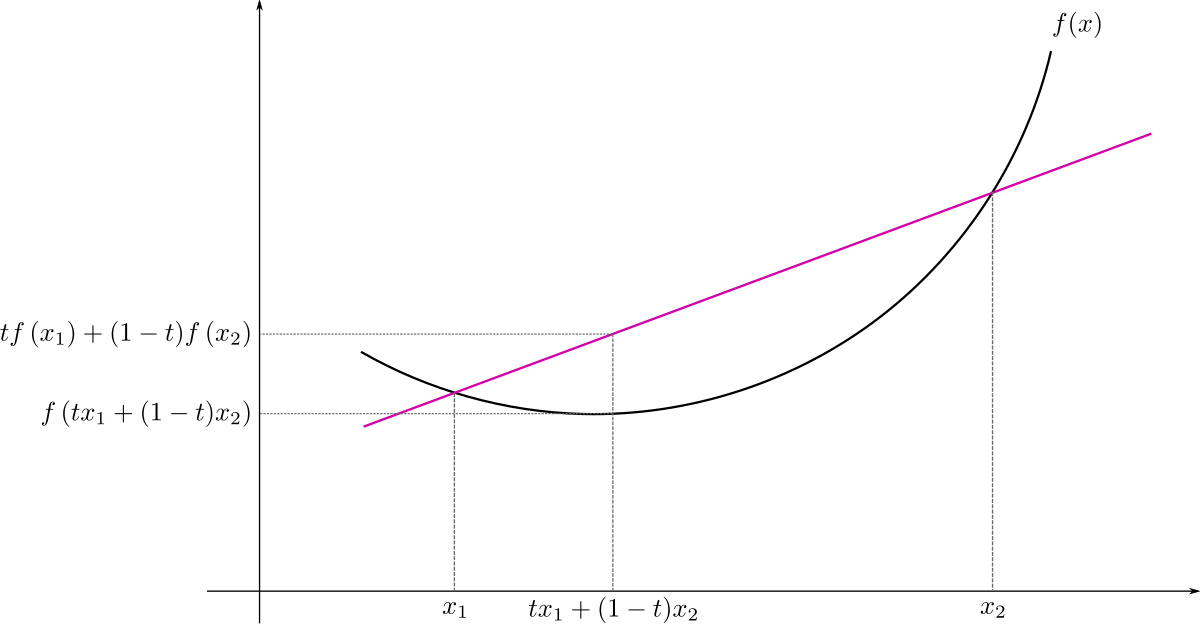
\includegraphics[width=0.8\textwidth]{5.convex}
\captionof{figure}{Convex function}
\label{fig:convex}}

\vspace{2mm}

For $1$-dimension function $f(x)$:

$$f(x) \ \ is \ \ convex \ \iff f''(x) \ge 0$$

\vspace{2mm}

\textbf{5.Differentiable in $(p,w)$}

* Higher-dimension proof not required in exam.

Recall one-dimension condition: derivative exists at $x^0 \Rightarrow$ Differentiable at $x^0$.


\vspace{3mm}
\textbf{6.Hotelling's lemma}

We already calculated the derivatives. Compare them with equation \ref{eq:E5} and \ref{eq:E6}.
%***************************************************
\subsection{Verify Theorem 3.8}

\begin{mdframed}[backgroundcolor=blue!20,linecolor=white]

\textbf{THEOREM 3.8 Properties of Output Supply and Input Demand Functions} (Jehle \& Reny pp.149)

Suppose that $f$ is a strictly concave production function satisfying Assumption 3.1 and that its associated profit function, $\pi(p, y)$, is twice continuously differentiable. Then, for all $p > 0$ and $w \gg 0$ where it is well defined:

\begin{enumerate}

\item Homogeneity of degree zero:
$$y(tp,tw) = y (p,w), \forall t > 0,$$
$$x_i(tp,tw) = x_i(p,w), \forall t > 0 \ and \  i = 1,\dots, n.$$
\item Own-price effects:
$$\frac{\partial y(p,w)}{\partial p} \ge 0,$$
$$\frac{\partial x_i(p,w)}{\partial w_i} \le 0, \ \forall i = 1,\dots, n. $$

\item The substitution matrix is symmetric and positive semidefinite.

\begin{equation}
\left(
    \begin{array}{cccc}
    \frac{\partial y(p,w)}{\partial p} & \frac{\partial y(p,w)}{\partial w_1} & \cdots & \frac{\partial y(p,w)}{\partial w_n} \\
    \frac{-\partial x_1(p,w)}{\partial p} & \frac{-\partial x_1(p,w)}{\partial w_1} & \cdots & \frac{-\partial x_1(p,w)}{\partial w_n} \\
    \vdots    &    \vdots & \ddots &   \vdots \\
    \frac{-\partial x_n(p,w)}{\partial p} & \frac{-\partial x_n(p,w)}{\partial w_1} & \cdots & \frac{-\partial x_n(p,w)}{\partial w_n} \\
    \end{array}
    \right)
\label{eq:subst}   
\end{equation}
\end{enumerate}
\end{mdframed}


Copy from Equation \ref{eq:E5}  and Equation \ref{eq:E6},

\textbf{Output supply function}:
$$
y(p,w) = (p\beta)^{-\frac{\beta}{\beta - 1}}(w_1^r + w_2^r)^{\frac{\beta}{r(\beta - 1)}}
$$

\textbf{Input demand function}:
$$
x_i(p,w) = w_i^{\frac{1}{\rho -1}}  (p\beta)^{\frac{-1}{\beta - 1}}(w_1^r + w_2^r)^{\frac{\rho -\beta}{\rho(\beta -1)}}
$$

\vspace{3mm}
\textbf{1.Homogeneity of degree zero}

\begin{align*}
y(tp,tw) &= (tp\beta)^{-\frac{\beta}{\beta - 1}}[(tw_1)^r + (tw_2)^r]^{\frac{\beta}{r(\beta - 1)}} \\
 &= t^{-\frac{\beta}{\beta - 1}}(p\beta)^{-\frac{\beta}{\beta - 1}} t^{\frac{\beta}{(\beta - 1)}} (w_1^r + w_2^r)^{\frac{\beta}{r(\beta - 1)}} \\
 &=t^0(p\beta)^{-\frac{\beta}{\beta - 1}}(w_1^r + w_2^r)^{\frac{\beta}{r(\beta - 1)}} \\
  &=t^0 y(p,w) 
\end{align*}

\begin{align*}
x_i(tp,tw) &= (tw_i)^{\frac{1}{\rho -1}}  (tp\beta)^{\frac{-1}{\beta - 1}}[(tw_1)^r + (tw_2)^r]^{\frac{\rho -\beta}{\rho(\beta -1)}} \\
&= t^{\frac{1}{\rho -1}} w_i^{\frac{1}{\rho -1}} t^{\frac{-1}{\beta -1}} (p\beta)^{\frac{-1}{\beta - 1}} t^{r\frac{\rho -\beta}{\rho(\beta -1)}} (w_1^r + w_2^r)^{\frac{\rho -\beta}{\rho(\beta -1)}} \\
 &=t^{\frac{1}{\rho -1} + \frac{-1}{\beta -1} + \frac{\rho}{\rho - 1}\frac{\rho -\beta}{\rho(\beta -1)}} w_i^{\frac{1}{\rho -1}}  (p\beta)^{\frac{-1}{\beta - 1}}(w_1^r + w_2^r)^{\frac{\rho -\beta}{\rho(\beta -1)}} \\
  &=t^0 x_i(p,w)
\end{align*}

$i = 1,2$.

\vspace{3mm}
\textbf{2.Own-price effects}

$$\frac{\partial y(p,w)}{\partial p} =(-\frac{\beta}{\beta - 1})p^{-\frac{\beta}{\beta - 1} - 1} (\beta)^{-\frac{\beta}{\beta - 1}}(w_1^r + w_2^r)^{\frac{\beta}{r(\beta - 1)}}$$

When $\beta \in (0,1), \frac{\partial y(p,w)}{\partial p} \ge 0$.

\begin{align*}
\frac{\partial x_i(p,w)}{\partial w_1} 
&=\frac{1}{\rho -1}w_1^{\frac{1}{\rho -1} -1} (p\beta)^{\frac{-1}{\beta - 1}}
(w_1^r + w_2^r)^{\frac{\rho -\beta}{\rho(\beta -1)}} +  
w_1^{\frac{1}{\rho -1}}  (p\beta)^{\frac{-1}{\beta - 1}} \frac{\rho -\beta}{\rho(\beta -1)}(w_1^r + w_2^r)^{\frac{\rho -\beta}{\rho(\beta -1)} -1} r w_1^{r -1} \\
&=\frac{1}{\rho -1}w_1^{\frac{1}{\rho -1} -1} (p\beta)^{\frac{-1}{\beta - 1}}
(w_1^r + w_2^r)^{\frac{\rho -\beta}{\rho(\beta -1)}} +  
w_1^{\frac{1}{\rho -1} + r -1}  (p\beta)^{\frac{-1}{\beta - 1}} \frac{\rho -\beta}{\rho(\beta -1)}(w_1^r + w_2^r)^{\frac{\rho -\beta}{\rho(\beta -1)} -1}  \frac{\rho}{\rho -1} \\
&=\frac{1}{\rho -1}w_1^{\frac{1}{\rho -1} -1} (p\beta)^{\frac{-1}{\beta - 1}}
(w_1^r + w_2^r)^{\frac{\rho -\beta}{\rho(\beta -1)}} +  
w_1^{\frac{1}{\rho -1} + r -1}  (p\beta)^{\frac{-1}{\beta - 1}} \frac{\rho -\beta}{(\rho -1)(\beta -1)}(w_1^r + w_2^r)^{\frac{\rho -\beta}{\rho(\beta -1)} -1}   \\
&= [\frac{1}{\rho -1} (w_1^r + w_2^r) + w_1^r \frac{\rho -\beta}{(\rho -1)(\beta -1)}] 
w_1^{\frac{1}{\rho -1} -1} (w_1^r + w_2^r)^{\frac{\rho -\beta}{\rho(\beta -1)} -1}(p\beta)^{\frac{-1}{\beta - 1}} \\
&= [(\frac{\beta -1}{(\rho -1)(\beta -1)} + \frac{\rho -\beta}{(\rho -1)(\beta -1)}) w_1^r + \frac{1}{\rho -1} w_2^r] 
w_1^{\frac{1}{\rho -1} -1} (w_1^r + w_2^r)^{\frac{\rho -\beta}{\rho(\beta -1)} -1}(p\beta)^{\frac{-1}{\beta - 1}} \\
&= [\frac{1}{\beta -1} w_1^r + \frac{1}{\rho -1} w_2^r] 
w_1^{\frac{1}{\rho -1} -1} (w_1^r + w_2^r)^{\frac{\rho -\beta}{\rho(\beta -1)} -1}(p\beta)^{\frac{-1}{\beta - 1}}
\end{align*}


Similarly, we have $$\frac{\partial x_i(p,w)}{\partial w_2} = [\frac{1}{\beta -1} w_1^r + \frac{1}{\rho -1} w_2^r] 
w_2^{\frac{1}{\rho -1} -1} (w_1^r + w_2^r)^{\frac{\rho -\beta}{\rho(\beta -1)} -1}(p\beta)^{\frac{-1}{\beta - 1}}
$$

When $\beta \in (0,1), \rho<1, \frac{\partial y(p,w)}{\partial w_i} \le 0$ ,$i = 1,2$.

\begin{mdframed}[backgroundcolor=yellow!20,linecolor=white]
1. Assign some value to the parameters and variables to verify your calculation:

\begin{itemize}
\item Let, for example, $p = 2, \rho = -1, \beta = 0.5, w_1 = w_2 = 2$, then $r =  \frac{\rho}{\rho -1} = 0.5 , \frac{\rho -\beta}{\rho(\beta -1)} = -3$
\item Calculate the first line of $\frac{\partial x_i(p,w)}{\partial w_1}$ and the simplified result in the last line, they should be the same ( $- \frac{5}{256}$)
\end{itemize}
2. In exam, leave it to the last if the calculation is very heavy and you find the result seems to be wrong.

3. We will NOT repeatedly punish you for wrong results, i.e., if the wrong results in step $1$ lead to mistakes in the rest steps, as long as your method is correct, you will get the point for the rest part. 

For example, a question asks you to calculate Elasticity of Substitution and  what substitution relationship the result implies.The correct answer is "$ES = + \infty$, perfect substitution". 
\begin{itemize}
\item   If you calculated it wrongly and have "$ES = 0$, no substitution", you will get points from "no substitution", the "correct" conclusion based on your wrong $ES$
\item   If you calculated it wrongly and have "$ES = 0$", but argue "$ES = 0$" implies "perfect substitution", then it's
totally wrong and you get no point, even though the conclusion "perfect substitution" is the same as the solution.
\end{itemize}

\end{mdframed}

\vspace{3mm}
\textbf{3.Substitution matrix}

Proof not really required in exam. But it may be helpful to understand it.

\begin{mdframed}[backgroundcolor=blue!20,linecolor=white]

According to Hotelling's lemma,
$$y(p,w) = \frac{\partial \pi(p,w)}{\partial p},\ and \ \ x_i(p,w) = - \frac{\partial \pi(p,w)}{\partial w_i}. \ \ \ \ i = 1,2, \dots , n.$$

We can rewrite:

$$\frac{\partial y(p,w)}{\partial p} = \frac{\partial^2 \pi(p,w)}{\partial p^2}$$
$$\frac{\partial y(p,w)}{\partial w_i} = \frac{\partial^2 \pi(p,w)}{\partial p \partial w_i}$$
$$-\frac{\partial x_i(p,w)}{\partial p} = \frac{\partial^2 \pi(p,w)}{\partial w_i \partial p }$$
$$-\frac{\partial x_i(p,w)}{\partial w_j} = \frac{\partial^2 \pi(p,w)}{\partial w_i \partial w_j}$$

The Substitution matrix is therefore the Hessian Matrix (check seminar 2) of the Profit Function $\pi(p,w)$:

\begin{equation}
\left(
    \begin{array}{cccc}
    \frac{\partial^2 \pi(p,w)}{\partial p^2} & \frac{\partial^2 \pi(p,w)}{\partial p \partial w_1} & \cdots & \frac{\partial^2 \pi(p,w)}{\partial p \partial w_n} \\
    \frac{\partial^2 \pi(p,w)}{\partial w_1 \partial p } & \frac{\partial^2 \pi(p,w)}{\partial w_1^2} & \cdots & \frac{\partial^2 \pi(p,w)}{\partial w_1 \partial w_n} \\
    \vdots    &    \vdots & \ddots &   \vdots \\
    \frac{\partial^2 \pi(p,w)}{\partial w_n \partial p } &  \frac{\partial^2 \pi(p,w)}{\partial w_n \partial w_1} & \cdots &  \frac{\partial^2 \pi(p,w)}{\partial w_n^2} \\
    \end{array}
    \right)
\label{eq:subst_s}   
\end{equation}


According to Young's theorem (Jehle \& Reny pp.557),$\frac{\partial^2 \pi(p,w)}{\partial p \partial w_i} = \frac{\partial^2 \pi(p,w)}{\partial w_i \partial p }$ , the matrix must be symmetric.

As a convex function, Profit Function $\pi(p,w)$ must have a positive semidefinite Hessian Matrix.

To prove the matrix is positive semidefinite is not required in exam, but you need to know the definition:

\textbf{Positive semidefinite}(Jehle \& Reny pp.559): a $n \times n$ metrix $A$ is positive semidefinite if for
all vectors $z \in R^n$, $z^TAz \ge 0$

Assume matrix $S$ is a Substitution matrix,
\begin{itemize}
\item Let $z = (1,0 , \dots, 0)^T$, $$z^T S z = \frac{\partial y(p,w)}{\partial p} \ge 0$$
\item Let $z = (0,1 , \dots, 0)^T$, $$z^T S z = \frac{-\partial x_1(p,w)}{\partial w_1}  \ge 0$$
\item $\dots$
\end{itemize}

\end{mdframed}

You can find the diagonal elements of a positive semidefinite matrix is always non-negative.

The conclusion above is the same as the so-called "Own-price effects" we have proved.
%%%%%%%%%%%%%%%%%%%%%%%%%%%%%%%%%%%%%%%%%%%%%%%%%%%%%%%%%%%%%%%%%%%%%%%%%%%%%%%%%%%%%%%%%%%%%%
\section{Jehle \& Reny 3.49}

\begin{enumerate}
\item Derive the \textbf{cost function} for the production function in Example 3.5 . 

\item Solve $\max_y py - c(w, y)$ 

\item Compare its solution, $y(p,w)$, to the solution in (E.5). Check that $\pi (p,w) = py(p,w) - c(w, y(p,w))$. 

\item Supposing that $\beta > 1$, confirm our conclusion that profits are minimised when the
first-order conditions are satisfied by showing that marginal cost is decreasing at the solution. 

\item Sketch your results.

\end{enumerate}

%***************************************************
\subsection{Cost function}

\begin{mdframed}[backgroundcolor=blue!20,linecolor=white]
CES  production function in Example 3.5 : $y = (x_1^\rho + x_2^\rho)^{\frac{\beta}{\rho}}$, $\beta < 1$ and $0 \ne \rho <1$

Cost function: $c(w,y) \equiv \min_{x \in \R^n_+} w \cdot x , \ \ s.t. \ \ f(x) \ge y.$
\end{mdframed}


$$c(w,y) = \min_{x \in \R^n_+} w_1x_1 + w_2x_2 , \ \ s.t. \ \ (x_1^\rho + x_2^\rho)^{\frac{\beta}{\rho}} \ge y$$

No corner solution.

\begin{itemize}
\item Obviously $x_1,x_2$ can't both be $0$ to produce $y>0$.
\item $\frac{\partial f(x)}{\partial x_i} = \beta (x_1^\rho + x_2^\rho)^{(\frac{\beta}{\rho}) - 1}x_i^{\rho - 1}$. If $\rho \in (0,1),\beta > 0$, $\lim_{x_i \to 0}\frac{\partial f(x)}{\partial x_i} = +\infty$. 
\begin{itemize}
\item If $\rho \in (0,1),\beta < 0$, the production function doesn't make sense since $\lim_{x \to (0,0)} f(x) = + \infty$
\item  If  $\rho < 0$, the production function is not defined at $x_i = 0$
\end{itemize}

\item $f(x) = y$ is binding: $f(x)$ is increasing in $x$, to reduce cost, we shouldn't produce more than required ($y$).
\end{itemize}

$$L =  w_1x_1 + w_2x_2 + \lambda [y -  (x_1^\rho + x_2^\rho)^{\frac{\beta}{\rho}}] $$ 

FOC:

\begin{equation}
    \begin{cases}
\frac{\partial L}{\partial x_1} =w_1 - \lambda \beta (x_1^\rho + x_2^\rho)^{(\frac{\beta}{\rho}) - 1}x_1^{\rho - 1}= 0 \\
\frac{\partial L}{\partial x_2} =w_2 - \lambda \beta (x_1^\rho + x_2^\rho)^{(\frac{\beta}{\rho}) - 1}x_2^{\rho - 1} = 0 \\
y -  (x_1^\rho + x_2^\rho)^{\frac{\beta}{\rho}} = 0
    \end{cases}
    \nonumber
\end{equation}

Simplify:

\begin{equation}
    \begin{cases}
 w_1 = \lambda \beta (x_1^\rho + x_2^\rho)^{(\frac{\beta}{\rho}) - 1}x_1^{\rho - 1} \\
 w_2 =\lambda \beta (x_1^\rho + x_2^\rho)^{(\frac{\beta}{\rho}) - 1}x_2^{\rho - 1} \\
(x_1^\rho + x_2^\rho)^{\frac{\beta}{\rho}} = y
    \end{cases}
    \label{eq:3_49_foc}   
\end{equation}

Taking the ratio between the first two gives:

$$\frac{w_1}{w_2}= (\frac{x_1}{x_2})^{\rho - 1} \Rightarrow x_1 = (\frac{w_1}{w_2})^{\frac{1}{\rho - 1}} x_2$$

Substituting in the third gives:

\begin{align*}
\{[(\frac{w_1}{w_2})^{\frac{1}{\rho - 1}} x_2]^\rho + x_2^\rho\}^{\frac{\beta}{\rho}} &=y \\
[(\frac{w_1}{w_2})^{\frac{\rho}{\rho - 1}} x_2^\rho + x_2^\rho]^{\frac{\beta}{\rho}} &=y \\
[(\frac{w_1}{w_2})^{\frac{\rho}{\rho - 1}} + 1]^{\frac{\beta}{\rho}} x_2^\beta &=y \\
x_2 &= (\frac{y}{[(\frac{w_1}{w_2})^{\frac{\rho}{\rho - 1}} + 1]^{\frac{\beta}{\rho}} })^{\frac{1}{\beta}} \\
 &= y^{\frac{1}{\beta}} [\frac{1}{(\frac{w_1}{w_2})^{\frac{\rho}{\rho - 1}} + 1}]^{\frac{1}{\rho}} \\
&= y^{\frac{1}{\beta}} [\frac{1}{(\frac{w_1}{w_2})^{\frac{\rho}{\rho - 1}} + 1}]^{\frac{1}{\rho}} \\
&= y^{\frac{1}{\beta}} (\frac{w_2^{\frac{\rho}{\rho - 1}}}{w_1^{\frac{\rho}{\rho - 1}} + w_2^{\frac{\rho}{\rho - 1}}})^{\frac{1}{\rho}} \\
\Rightarrow x_1 &= (\frac{w_1}{w_2})^{\frac{1}{\rho - 1}} x_2  \\
&= y^{\frac{1}{\beta}} (\frac{w_1^{\frac{\rho}{\rho - 1}}   }{w_2^{\frac{\rho}{\rho - 1}}   } \frac{w_2^{\frac{\rho}{\rho - 1}}}{w_1^{\frac{\rho}{\rho - 1}} + w_2^{\frac{\rho}{\rho - 1}}})^{\frac{1}{\rho}}  \\
&=y^{\frac{1}{\beta}} (\frac{w_1^{\frac{\rho}{\rho - 1}}}{w_1^{\frac{\rho}{\rho - 1}} + w_2^{\frac{\rho}{\rho - 1}}})^{\frac{1}{\rho}} 
\end{align*}

Cost function: 
\begin{align*}
c(w,y) = w_1x_1 + w_2x_2 &= w_1y^{\frac{1}{\beta}} (\frac{w_1^{\frac{\rho}{\rho - 1}}}{w_1^{\frac{\rho}{\rho - 1}} + w_2^{\frac{\rho}{\rho - 1}}})^{\frac{1}{\rho}}  +w_2 y^{\frac{1}{\beta}} (\frac{w_2^{\frac{\rho}{\rho - 1}}}{w_1^{\frac{\rho}{\rho - 1}} + w_2^{\frac{\rho}{\rho - 1}}})^{\frac{1}{\rho}} \\
&= w_1y^{\frac{1}{\beta}} \frac{w_1^{\frac{1}{\rho - 1}}}{(w_1^{\frac{\rho}{\rho - 1}} + w_2^{\frac{\rho}{\rho - 1}})^{\frac{1}{\rho}}}  +w_2 y^{\frac{1}{\beta}} \frac{w_2^{\frac{1}{\rho - 1}}}{(w_1^{\frac{\rho}{\rho - 1}} + w_2^{\frac{\rho}{\rho - 1}})^{\frac{1}{\rho}}} \\
&=y^{\frac{1}{\beta}} [\frac{w_1^{(\frac{1}{\rho - 1}+1)}}{(w_1^{\frac{\rho}{\rho - 1}} + w_2^{\frac{\rho}{\rho - 1}})^{\frac{1}{\rho}}} + \frac{w_2^{(\frac{1}{\rho - 1}+1)}}{(w_1^{\frac{\rho}{\rho - 1}} + w_2^{\frac{\rho}{\rho - 1}})^{\frac{1}{\rho}}}] \\
&=y^{\frac{1}{\beta}}\frac{w_1^r+w_1^r}{(w_1^r + w_2^r)^{\frac{1}{\rho}}} \\
&=y^{\frac{1}{\beta}}{(w_1^r + w_2^r)^{1 - \frac{1}{\rho}}} \\
&=y^{\frac{1}{\beta}}{(w_1^r + w_2^r)^{\frac{1}{r}}} \\
\end{align*}

Where $r = \frac{\rho}{\rho -1}$

%***************************************************
\subsection{Solve $\max_y py - c(w, y)$ }

\begin{mdframed}[backgroundcolor=blue!20,linecolor=white]

We already know the cost function given output $y$:
$$c(w,y) = y^{\frac{1}{\beta}}{(w_1^r + w_2^r)^{\frac{1}{r}}} $$

Forget that we already know \textbf{Profit maximization $\Rightarrow$  Cost minimization} for now.

To maximize our profit, we want instead the difference between $py$ and $c(w,y)$ \\ (the least cost for every given $y$) to be as big as possible,i.e.:
$$\max_{y} py - c(w,y)$$

As a price receiver (competitive firm), how should we change $y$ to achieve this?

If you're sure there is only one solution, and the question asks you to find the maximum point, then FOC is enough:

$$\frac{d(py - c(w,y))}{dy} = p - \frac{dc(w,y)}{dy}=0$$


\end{mdframed}

$$py - c(w, y) = py - y^{\frac{1}{\beta}}{(w_1^r + w_2^r)^{\frac{1}{r}}} $$

FOC:

$$\frac{d(py - y^{\frac{1}{\beta}}{(w_1^r + w_2^r)^{\frac{1}{r}}})}{dy}= p - \frac{1}{\beta}y^{\frac{1}{\beta} - 1} (w_1^r + w_2^r)^{\frac{1}{r}} = 0$$

\begin{equation}
\therefore y^{\frac{1- \beta}{\beta}} = p \beta (w_1^r + w_2^r)^{-\frac{1}{r}}  \Rightarrow y =  (p \beta)^{\frac{\beta}{1- \beta}} (w_1^r + w_2^r)^{^{\frac{\beta}{r(\beta - 1)}}}
    \label{eq:check1}   
\end{equation}

%***************************************************
\subsection{Compare with profit maximization problem}

\textbf{1.Output function}

Compare the output function \ref{eq:check1} with function \ref{eq:E5}, the results are the same.

\textbf{1.Profit function}

\begin{align}
\begin{split}
py(p,w) - c(w, y(p,w)) &= p[(p \beta)^{\frac{\beta}{1- \beta}} (w_1^r + w_2^r)^{^{\frac{\beta}{r(\beta - 1)}}}] \\ 
&\ \ \ \ \ \ \ \ - [(p \beta)^{\frac{\beta}{1- \beta}} (w_1^r + w_2^r)^{^{\frac{\beta}{r(\beta - 1)}}}]^{\frac{1}{\beta}}{(w_1^r + w_2^r)^{\frac{1}{r}}} \\
&= p^{\frac{1}{1- \beta}} \beta^{\frac{\beta}{1- \beta}}(w_1^r + w_2^r)^{^{\frac{\beta}{r(\beta - 1)}}} \\ 
&\ \ \ \ \ \ \ \ - (p\beta)^{\frac{1}{1- \beta}} (w_1^r + w_2^r)^{\frac{1}{r(\beta - 1)}}(w_1^r + w_2^r)^{\frac{1}{r}} \\
&= p^{\frac{1}{1- \beta}} \beta^{\frac{\beta}{1- \beta}}(w_1^r + w_2^r)^{^{\frac{\beta}{r(\beta - 1)}}} - (p\beta)^{\frac{1}{1- \beta}} (w_1^r + w_2^r)^{\frac{\beta}{r(\beta - 1)}} \\
&= [p^{\frac{1}{1- \beta}} \beta^{\frac{\beta}{1- \beta}} - (p\beta)^{\frac{1}{1- \beta}}] (w_1^r + w_2^r)^{\frac{\beta}{r(\beta - 1)}} \\
&= [p^{\frac{1}{1- \beta}} \beta^{\frac{\beta}{1- \beta}} - p^{\frac{1}{1- \beta}} \beta^{\frac{1}{1- \beta}}] (w_1^r + w_2^r)^{\frac{\beta}{r(\beta - 1)}} \\
&= [ \beta^{\frac{\beta}{1- \beta}} -\beta^{\frac{1}{1- \beta}}] p^{\frac{1}{1- \beta}}(w_1^r + w_2^r)^{\frac{\beta}{r(\beta - 1)}} \\
&= [ 1 -\beta^1] \beta^{\frac{\beta}{1- \beta}} p^{\frac{1}{1- \beta}}(w_1^r + w_2^r)^{\frac{\beta}{r(\beta - 1)}} \\
&= p^{\frac{1}{1- \beta}}(w_1^r + w_2^r)^{\frac{\beta}{r(\beta - 1)}} \beta^{\frac{\beta}{1- \beta}}(1 -\beta^1)
\end{split}
\label{eq:check2}   
\end{align}

Compare the result \ref{eq:check2} with the profit function \ref{eq:E7} obtained from profit maximization problem.

\begin{center}
\textbf{Profit maximization $\iff$  Cost minimization(+one more step)}
\end{center}

%***************************************************
\subsection{Marginal Cost and output}

\begin{mdframed}[backgroundcolor=blue!20,linecolor=white]

FOC may be not enough:

\begin{itemize}
\item FOC is not sufficient for maximum/minimum point (sometimes it is \href{https://en.wikipedia.org/wiki/Inflection_point}{Inflection Point}).
\item When FOC has more than 2 solutions, FOC is not enough to determine which is the local maximum/minimum point.
\end{itemize}

\vspace{2mm}

Figure \ref{fig:soc} is a very nice plot showing why FOC is not enough for "maximum poit":

\vspace{2mm}
{\centering
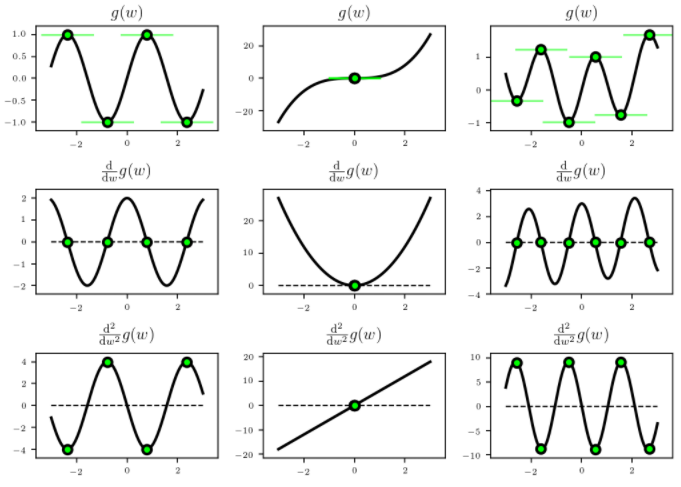
\includegraphics[width=0.8\textwidth]{5.soc}
\captionof{figure}{Second order condition}
\label{fig:soc}}
\vspace{2mm}

(The Figure is from \href{https://kenndanielso.github.io/mlrefined/blog_posts/7_Second_order_methods/7_8_Second_order_condition.html}{Intuiting the condition by example})

\vspace{3mm}

We therefore need to check SOC:

$$\frac{d^2(py - c(w,y))}{dy^2} = - \frac{d^2c(w,y)}{dy^2} \le 0 \Rightarrow \frac{d^2c(w,y)}{dy^2} \ge 0$$

\vspace{3mm}

To sum up:


(1) By FOC, we choose the level $y^*$ of output such that 
$$\frac{dc(w,y)}{dy}= p$$
(Marginal cost = price). And,

(2) By SOC, we also require 

$$\frac{d^2c(w,y)}{dy^2} = MC \ge 0$$

(Marginal cost increasing in scale)


\vspace{2mm}
{\centering
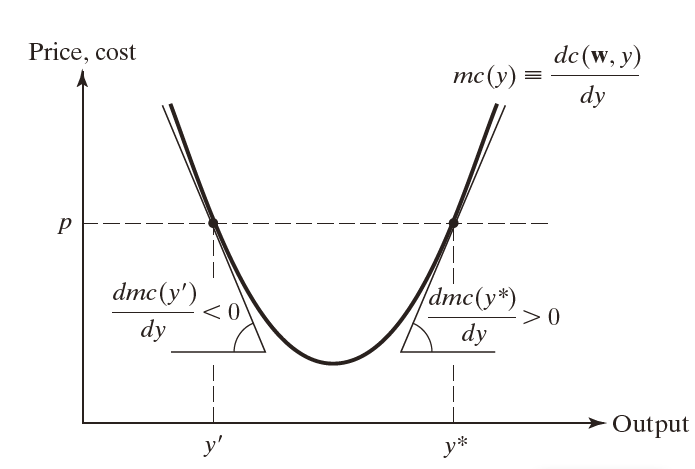
\includegraphics[width=0.8\textwidth]{5.mc}
\captionof{figure}{Marginal cost and price}
\label{fig:mc}}
\vspace{2mm}

\end{mdframed}

Given $c(w,y) = y^{\frac{1}{\beta}}{(w_1^r + w_2^r)^{\frac{1}{r}}} $,

$$MC=\frac{dc(w,y)}{dy}= \frac{1}{\beta}  y^{\frac{1}{\beta} - 1}{(w_1^r + w_2^r)^{\frac{1}{r}}}$$

$$\frac{d MC}{dy} = \frac{1}{\beta}(\frac{1}{\beta} - 1)  y^{\frac{1}{\beta} - 2}{(w_1^r + w_2^r)^{\frac{1}{r}}}$$


If $\beta >1$, $\frac{d MC}{dy} < 0$. The solution is therefore minimized profit, instead of maximized profit.

\begin{mdframed}[backgroundcolor=blue!20,linecolor=white]
Intuitively, $MC=\frac{1}{\beta}  y^{\frac{1}{\beta} - 1}{(w_1^r + w_2^r)^{\frac{1}{r}}}$ is decreasing in $y$ when $\beta > 1$, the more you produce, the less cost you need to pay for 1 more unit output. You will therefore continue to produce $+\infty$.

\end{mdframed}

%***************************************************
\subsection{Sketch}

\begin{center}
\begin{tikzpicture}[scale=1]
\draw[thick,<->] (0,7) node[left]{$\$$}--(0,0)--(10,0) node[right]{$y$};
\node [below left] at (0,0) {$0$};
\draw(1,6) ..controls (2,5) and (5,3).. (9,3) node[right]{$MC$};
\draw [blue] (0,4)--(10,4) ;
\draw (4.16,0)--(4.16,4) ;
\node[left,blue] at (0,4) {$p$} ;
\node[below] at (4.16,0) {$y^*$} ;

\end{tikzpicture}
\captionof{figure}{Decreasing MC and p}
\label{fig:mc}
\end{center}
\vspace{2mm}

If you stop at $y^*$, you lose the most!

\end{document}
